\documentclass[mathserif]{beamer}
\usepackage{beamerthemeshadow}
\usepackage{beamerthemesplit}
%\usetheme{shadow}
\usecolortheme{default}
\setbeamertemplate{footline}[frame number]
\useinnertheme[shadow=true]{rounded}
%\setbeamertemplate{footline}{\insertframenumber/\inserttotalframenumber}
%\useoutertheme{infolines}
%\setbeamertemplate{headline}{} % removes the headline that infolines inserts

%\usetheme{boxes}
%\usepackage{amsmass}
%\usepackage{amssymb,amsfonts,url}


\usepackage{algorithm}
\usepackage{algorithmic}

\usepackage{graphicx}
\graphicspath{{Problems/}}
\usepackage{subfigure}


\title{CS711008Z  Algorithm Design and Analysis }
\subtitle{ Lecture 2. Analysis techniques 
%\footnote{The slides are made based on Ch. 17 of Introduction to Algorithms, and Ch. 2 of Algorithm Design. Some slides are excerpted from Kevin Wayne's slides with permission. }
}
\author{Dongbo Bu \\
\ \ \ \ \ \ \ \ \ \ \ \ \ \ \ \ \ \ \ \ \ \ \ \ \ \ \ \ \ \ \ \ \ \ \ \ \ \ \ \ \ \ \ \ \ \ \ \ \ \ \ \ \ \ \ \ \ \ \ \ \ \ \ \ \ \ \ \ \ \ \ \ \ \ \ \ \ \ \ \ \ \ \ \ \ \ \ \ \ \ \ \ \ \ \ \ \ \ \ \  \\
{\small Institute of Computing Technology \\ Chinese Academy of Sciences, Beijing, China}}
\date{}


\begin{document}
%\begin{CJK}{UTF8}{cyberbit}

\frame{\titlepage}

%\section[Outline]{}
%\frame{\tableofcontents}

%    \begin{figure}
%        \centering
%        \includegraphics[width=0.8\textwidth]{newGeneRep.eps}
%    \end{figure}

% \begin{figure}%
%   \begin{center}%
%     \begin{minipage}{0.70\textwidth}%
%      \includegraphics[width=1.0\textwidth]{comp25000.eps}%
%     \end{minipage}%
%     \begin{minipage}{0.30\textwidth}
%      \includegraphics[width=1.0\textwidth]{comparelabel.eps}%
%     \end{minipage}%
%   \end{center}
% \end{figure}

% \begin{table}
%   {\begin{tabular}{l|rrr}\hline
%       & \multicolumn{3}{c}{Actual number of DCJ operations}\\
%       \# genes &\# genes $\times 1$&\# genes $\times 2$&\# genes  $\times 3$ \\
% \hline
%      (a)~25,000 & 0.5\% ~~&  0.9\% ~~& 1.7\%~~\\
%       (b)~10,000 & 0.8\%~~ &  1.4\% ~~& 2.7\%~~\\
%      (c)~ 1,000 & 2.7\%~~ & 4.7\%~~ & 14.7\%~~\\ \hline
%     \end{tabular}} {}%
% \end{table}

\frame{
\frametitle{What is efficiency?}
\begin{itemize}
 \item 
{\bf Definition 1:} An algorithm is efficient if, when implemented, it runs quickly on
real input instances.  
\item 
{\bf Questions: }
\begin{itemize}
\item  What is the platform? \\
\item  Is the algorithm implemented well? \\
 \item What is a ``real'' instance?  \\
 \item How well, or badly, does the algorithm scale with the instance size? 
 \item Both $Algo1$ and $Algo2$ perform well for a small instance; however, on a larger instance, one algorithm may be still fast, while the other one are very slow; 
\end{itemize}
\end{itemize}
}

\frame{
\frametitle{What is efficiency? cont'd }
\begin{itemize}
 \item 
{\bf Definition 2:} An algorithm is efficient if it achieves qualitatively better
worst-case performance, at an analytical level, than brute-force search. 
\item 
{\bf Questions: }
\begin{itemize}
\item 
 Good: Algorithms better than brute-force search nearly always contains a valuable idea to make it work, and tell us the something about the intrinsic structure. \\
 \item 
Bad: ``quantatively'' requires the actual running time of algorithm; thus, we should derive the running time carefully. \\
 \end{itemize}
 \end{itemize}

 

}


\frame{
\frametitle{What is efficiency? cont'd }
\begin{itemize}
 \item 
{\bf Definition 3:} An algorithm is efficient if it has a polynomial worst-case
running time (known as Cobham-Edmonds thesis)
\item 
{\bf Justification:} It really works in practice. 
\begin{itemize}
 \item In practice, the polynomial time algorithm that people develop almost 
always have low constant and low exponents; \\
\item  Breaking the exponential barrier of brute-force usually means 
the exposition of problem structure. 
\end{itemize}
 \item  {\bf Exceptions: }
\begin{itemize}
 \item 
Some polynomial-time algorithms have a high constant or high exponents, thus unpractical. \\
\item 
Some exponential-time algorithms work well in practice since the worst-case is rare. 
\end{itemize}
 \end{itemize}
 
}

\frame{
  \frametitle{Algorithm analysis}
    \begin{enumerate}
     \item {\bf Worst-case analysis:} the largest possible time on a problem instance with size $n$; 
     \item {\bf Average-case analysis:} analyse average running time over all inputs
with a known distribution;  
     \item {\bf Amortized analysis:} worst case bound on \textcolor{red}{a sequence of operations}; 
    \end{enumerate}
    Note: Running time is usually measured in terms of elementary operations, say \textcolor{blue}{\bf  comparison} in sort algorithm. Intuitively, an elementary operation takes 1 unit time, and the running time is measured using the number of elementary operations. 
}

\frame{ 
  \begin{block}{}
    Average-case analysis 
  \end{block}
} 

\frame{
  \frametitle{Average-case analysis }
  \begin{itemize}
   \item Objective: analyze average running time over a distribution of inputs 
   
   \item Example: {\sc QuickSort} 
      \begin{enumerate}
       \item Worst-case complexity: $O(n^2)$  
       \item Average-case complexity: $O(n\log n)$  if input is
uniformly random
      \end{enumerate}
  \end{itemize}
  
%  Note: 
%  \begin{itemize}
%  \item Relationship between average-case complexity and randomized
%algorithm: leads to a randomized
%algorithm with an expectation time of $O(n\log n)$ 
%  \item 
%    However, it is usually not easy to know the actual distribution of inputs in
%practice 
%  \end{itemize}
}

\frame{
\frametitle{ An example }

{\bf Input:}  an array $A[1..n]$ of numbers  \\
{\bf Output:}  sorted array \\

 {\sc QuickSort} algorithm \\
\begin{algorithmic}[1]
\STATE  Pick an element, say the first element,  from $A$. This element is
called a pivot; 
\STATE  Partition $A$ into two sub-lists, one consisting of elements less than
the pivot, and another one consisting of elements larger than the pivot; 
\STATE   Recursively sort the sub-list of lesser elements and the sub-list of
greater elements.
\end{algorithmic}

}

\frame{
\frametitle{Best-case } 
\begin{itemize}
 \item The most balanced case: partitioning $A$ into two sub-lists of size $\frac{n}{2}$. 
% \item Time: $T(n)=O(n)+2T(\frac{n}{2}) = O(n\log n)$ 
 \end{itemize}
\begin{figure}
        \centering
        \includegraphics[width=2.1in]{L2-bestcasestep1.eps}
\end{figure}
}

\frame{
\frametitle{Best-case } 
\begin{itemize}
 \item The most balanced case: partitioning $A$ into two sub-lists of size $\frac{n}{2}$. 
 \end{itemize}
\begin{figure}
        \centering
        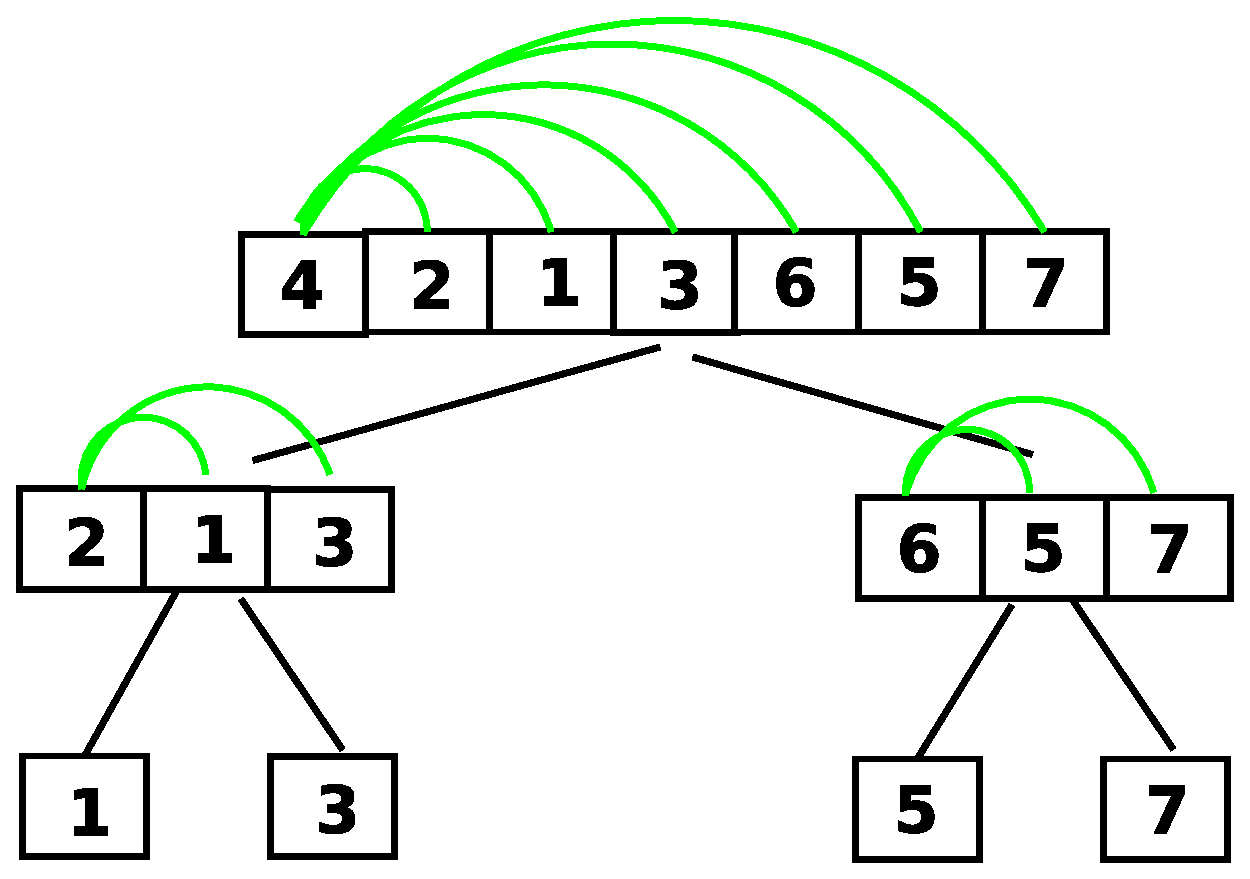
\includegraphics[width=2.1in]{L2-bestcasestep2.eps}
\end{figure}
Time: $T(n)=O(n)+2T(\frac{n}{2}) = O(n\log_{2} n)$ 

}

\frame{
\frametitle{Worst-case } 
\begin{itemize}
 \item The most unbalanced case: partitioning $A$ into two sub-lists with size 
1 and $n-1$. 
% \item Time: $T(n)=O(n)+T(n-1) = O(n^2)$ 
 \end{itemize}
\begin{figure}
        \centering
        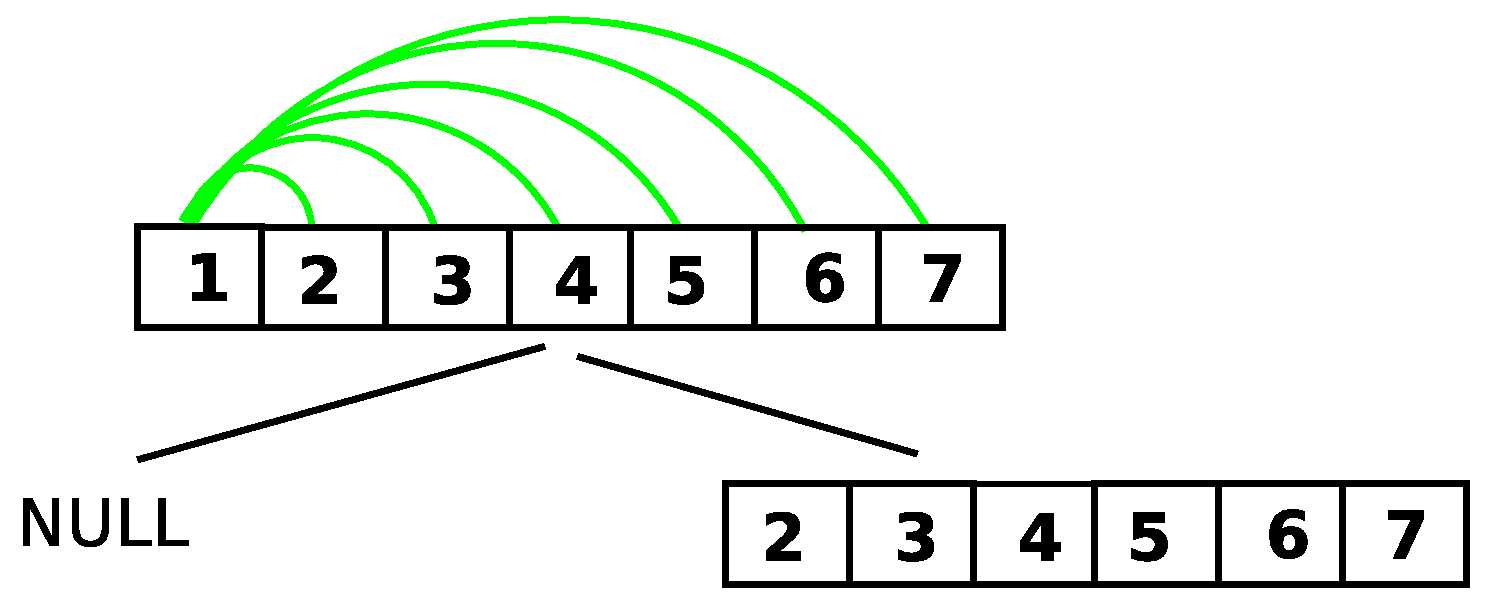
\includegraphics[width=2.4in]{L2-worstcasestep1.eps}
\end{figure}
 }
 
 \frame{
\frametitle{Worst-case } 
\begin{itemize}
 \item The most unbalanced case: partitioning $A$ into two sub-lists with size 
1 and $n-1$. 
% \item Time: $T(n)=O(n)+T(n-1) = O(n^2)$ 
 \end{itemize}
\begin{figure}
        \centering
        \includegraphics[width=3in]{L2-worstcasestep2.eps}
\end{figure}
 }

 \frame{
\frametitle{Worst-case } 
\begin{itemize}
 \item The most unbalanced case: partitioning $A$ into two sub-lists with size 
1 and $n-1$. 
% \item Time: $T(n)=O(n)+T(n-1) = O(n^2)$ 
 \end{itemize}
\begin{figure}
        \centering
        \includegraphics[width=3.4in]{L2-worstcasestep3.eps}
\end{figure}
 }
 
  \frame{
\frametitle{Worst-case } 

\begin{figure}
        \centering
        \includegraphics[width=4.6in]{L2-worstcasestep7.eps}
\end{figure}
Time: $T(n)=O(n)+T(n-1) = O(n^2)$ 

 }
 
 \frame{
 \frametitle{ Average-case } 
 \begin{itemize}
  \item Assumption:  the input is a random permutation
  \begin{figure}
        \centering
        \includegraphics[width=3in]{L2-averagecase0.eps}
\end{figure}
  \item Objective: what is the average cost? 
  \end{itemize} 


} 

 \frame{
 \frametitle{ Average-case } 
 \begin{figure}
        \centering
        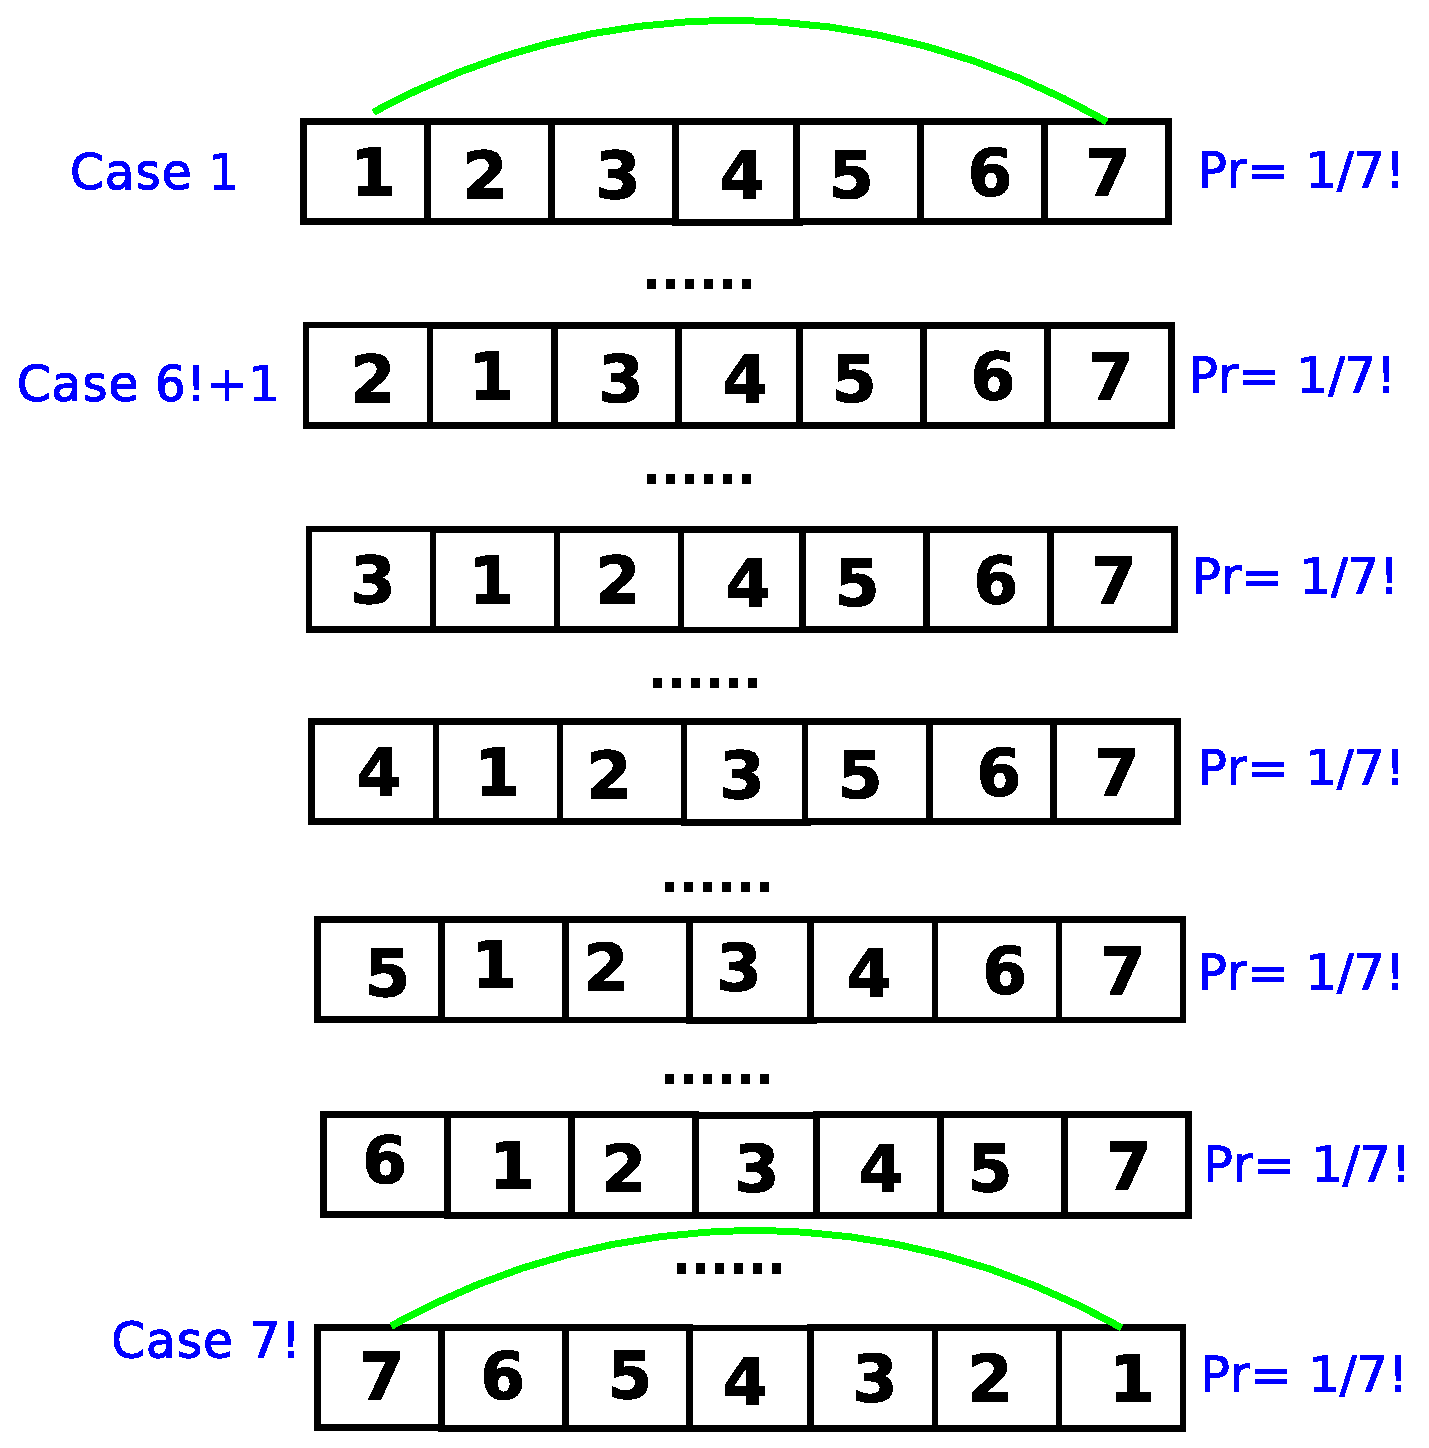
\includegraphics[width=2.4in]{L2-averagecase.eps}
\end{figure}
 \begin{itemize}
  \item Note that $\Pr( \text{1 compared with 7} ) = \frac{2}{7}$. Why? 
  \item In general, we have $\Pr( \text{ i compared with j } ) = \frac{2}{j-i+1}$
 \end{itemize}
 } 
 
 \frame{
 \frametitle{ Consider every pair } 
  \begin{eqnarray} 
  E( \#Comparison ) &=& \sum_{i=1}^{n-1} \sum_{j=i+1}^{n} \frac{2}{j-i+1}    \\ 
   &=& \sum_{i=1}^{n-1} \sum_{k=1}^{n-i} \frac{2}{k+1}    \\ 
   &<& \sum_{i=1}^{n-1} \sum_{k=1}^{n}  \frac{2}{k}  \\ 
   &\approx & 2 n \ln n  \\ 
   &\approx & 1.39 n \log_{2} n 
     \end{eqnarray} 
  
  Note: 
  \begin{itemize}
  \item Equation (2) comes from introducing an auxiliary variable $k=j-i$. 
  \item This means that, on average, {\sc QuickSort}  performs only about $39\%$ worse
than in its best case.
  \end{itemize}

  
 
}


\frame{ 
  \begin{block}{}
    Amortized  analysis 
  \end{block}
} 


\frame{
\frametitle{Amortized analysis}

\begin{itemize}
  \item Motivation: given a \textcolor{red}{ {\bf sequence} } of operations, the vast majority of the operations are cheap, but some rare operations within the sequence might be expensive; thus a standard worst-case analysis might be overly pessimistic. 
  \item Objective: to give a tighter bound for a  \textcolor{red}{ {\bf sequence} }  of operations.
  \item Basic idea: when the expensive operations are particularly rare, their costs can be ``spread out'' (amortized) to all operations. If the artificial amortized costs are still cheap, we will have a tighter bound of the whole sequence of operations. 
  \item Example: serving coffee in a bar  
 \end{itemize}
} 

\frame{
\frametitle{Amortized analysis versus average-case analysis}

Amortized analysis differs from average-case analysis in: 
	\begin{itemize}
		\item Average-case analysis: \textcolor{red}{ {\bf average over    all input} } , e.g., {\sc QuickSort} algorithm performs well on ``average'' over all possible input even if it performs very badly on certain input. 
		\item Amortized analysis: \textcolor{red}{ {\bf average over  operations} } , e.g., {\sc TableInsertion} algorithm performs well on ``average'' over all operations even if some operations use a lot of time.  
	\end{itemize}
}

\frame{
	\begin{block}{}
	 Stack with {\sc MultiPop} operation
	 \end{block}
}

\frame{
\frametitle{Problem: A Stack  with {\sc MultiPop} operation } 

Input: an array $A[1..n]$, an integer $K$; \\
A sequence of $n$ operations:  \\
\begin{algorithmic}[1]
\FOR{$i=1$ to $n$} 
\IF{ $A[i] \ge A[i-1]$ }
\STATE {\sc Push}($A[i]$); 
\ELSIF{ $A[i] \le A[i-1] - K$ }
\STATE {\sc MultiPop}( S, K );
\ELSE{}
\STATE {\sc Pop}();
\ENDIF
\ENDFOR
\end{algorithmic}

 {\sc MultiPop(S, k)}
\begin{algorithmic}[1]
\WHILE{ $S$ is not empty and $k > 0$ }
\STATE {\sc Pop}(S);
\STATE $k--$;
\ENDWHILE
\end{algorithmic} 
}

\frame{
\frametitle{ An example} 
\begin{figure}
        \centering
        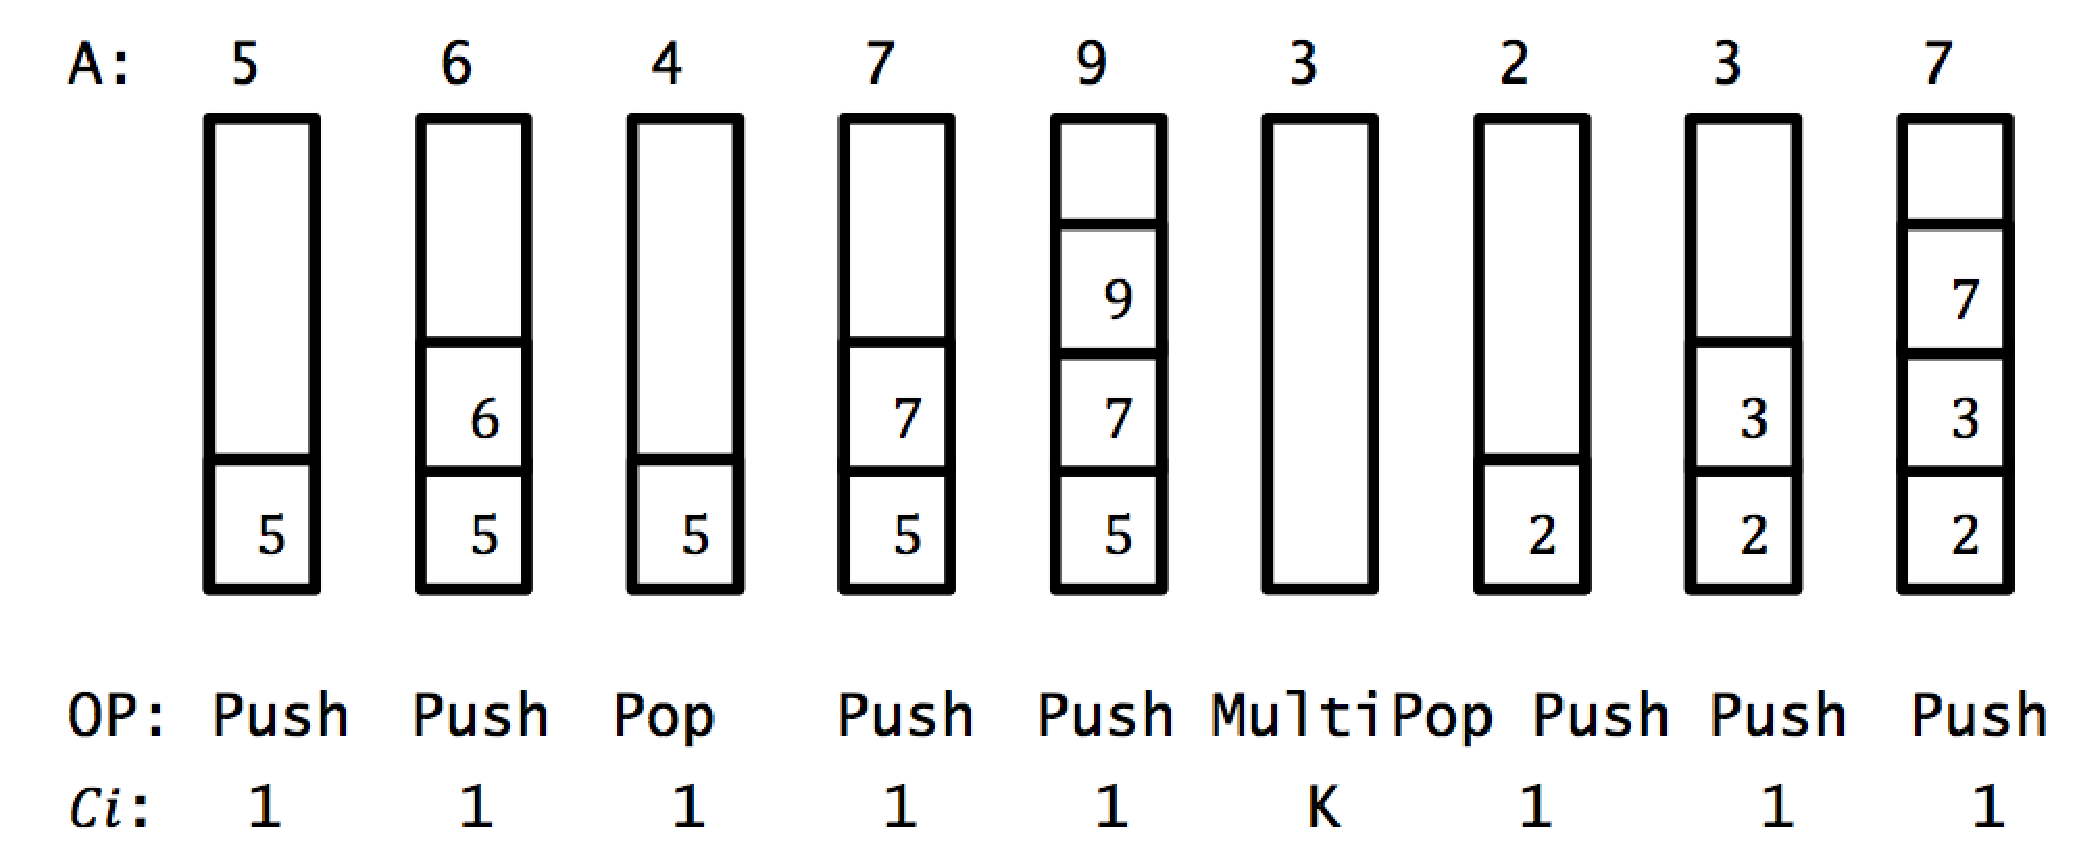
\includegraphics[width=3.5in]{L2-stackexample.eps}
\end{figure}

\begin{block}{Objective}
 For each operation assign an  \textcolor{red}{ {\bf amortized cost} }  $\widehat{C_{i}}$ to bound the actual total cost. 
 \end{block}
 
 
 In other words, we need to show that  for \textcolor{red}{ {\bf any sequence of $n$ operations}},  we have $T(n)=\sum_{i=1}^n C_i \leq  \sum_{i=1}^n  \widehat{C_{i}} $. Here, $C_{i}$ denotes the  \textcolor{red}{ {\bf actual cost}}   of step $i$.  

}

\frame{
\frametitle{Cursory analysis versus tighter analysis }

\begin{itemize}
 \item In a sequence of operations, some operations may be cheap, but some operations may be expensive, say   {\sc MultiPop()}. 
\item
Cursory analysis: {\sc MultiPop()} step may take $O(n)$ time; thus,
 $T(n) = \sum_{i=1}^n C_i \le  n^{2} $  

 \item However, the worst operation does not occur often.  
\item Therefore, the traditional worst-case  \textcolor{red}{ {\bf individual operation} }  analysis can give overly
pessimistic bound. 
\end{itemize}
} 

%\frame{
%\framettile{ Tighter bound: amortized analysis } 
%Tighter analysis: 
%\begin{itemize}
%\item Aggregate technique: all operations have the same {\sc amortized cost} $\frac{1}{n} \sum_{i=1}^{n} \widehat{C_{i}}$. 
%\item Accounting technique: when there is more than one type of operation, each type of operation might be assigned with different amortized cost. If $\widehat{C_{i}} > C_{i}$, the overcharge will be stored as ``prepaid credit''; the credit will be used later for the operations with $\widehat{C_{i}} < C_{i}$. 
% \item Potential technique: Using ``potential function'' as a bridge to set $\widehat{C_{i}}$. 
%\end{itemize}
%}

\frame{
	\begin{block}{}
	Tighter analysis 1: aggregate technique 
	 \end{block}
}

\frame{
\frametitle{Tighter analysis 1: Aggregate technique }
\begin{itemize}
\item Basic idea: all operations have the same {\sc amortized cost} $\frac{1}{n} \sum_{i=1}^{n} \widehat{C_{i}}$
\item Key observation: $\# Pop \le \#Push$ \\
\item Thus, we have: 
\begin{eqnarray}
T(n) &=&  \sum_{i=1}^n C_i \\
     &=&  \# Push + \#Pop \\
     &\le & 2\times \#Push \\
     &\le & 2n 
\end{eqnarray}
\item 
On average, the $MultiPop(K)$ step takes only $O(1)$ time rather than $O(K)$ time. 
\end{itemize}

}


\frame{
	\begin{block}{}
	Tighter analysis 2: accounting technique 
	 \end{block}
}

\frame{
\frametitle{ Tighter analysis 2: Accounting technique  }

\begin{itemize}
 \item 
Basic idea: for each operation $OP$ with actual cost $C_{OP}$, an amortized cost $\widehat{C_{OP}}$ is assigned such that for \textcolor{red}{\bf any sequence of $n$ operations},  $T(n) = \sum_{i=1}^n C_i \le  \sum_{i=1}^n \widehat{C_i}$.
\item Intuition:  If $\widehat{C_{op}} > C_{op}$, the overcharge will be stored as  \textcolor{red}{ {\bf prepaid credit}}; the credit will be used later for the operations with $\widehat{C_{op}} < C_{op}$.  The requirement that $ \sum_{i=1}^n C_i \le  \sum_{i=1}^n \widehat{C_i}$ is essentially \textcolor{red}{\bf credit never goes negative.} 
\item Example: 
\begin{small} 
 \begin{table}
   {\begin{tabular}{r|c|c}
       OP & Real Cost $C_{op}$ & Amortized Cost $\widehat{C_{op}}$ \\ \hline
       {\sc Push} & 1 & 2 \\ 
       {\sc Pop } & 1 & 0 \\ 
       {\sc MultiPop} & $k$ & 0 \\
            \end{tabular}} {}%
 \end{table}
 \end{small}
 \item Credit:  the number of items in the stack.
\end{itemize} 
 } 
 
 \frame{
\frametitle{ Tighter analysis 2: Accounting technique  }

\begin{itemize}
%\begin{figure}
%        \centering
%        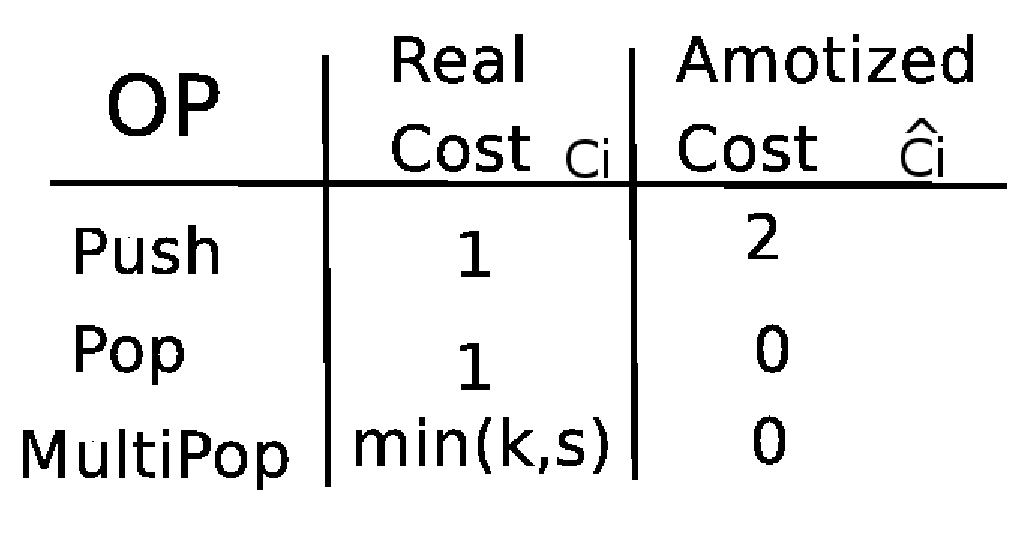
\includegraphics[width=1.5in]{L2-stackaccounting.eps}
%\end{figure}
\item Example: 
\begin{small} 
 \begin{table}
   {\begin{tabular}{r|c|c}
       OP & Real Cost $C_{op}$ & Amortized Cost $\widehat{C_{op}}$ \\ \hline
       {\sc Push} & 1 & 2 \\ 
       {\sc Pop } & 1 & 0 \\ 
       {\sc MultiPop} & $k$ & 0 \\
            \end{tabular}} {}%
 \end{table}
 \end{small}

\item In summary, starting from an empty stack, \textcolor{red}{ {\bf any } } sequence of $n_{1}$ {\sc Push}, $n_{2}$ {\sc Pop}, and $n_{3}$ {\sc MultiPop} operations takes at most $T(n) = \sum_{i=1}^n C_i \le   \sum_{i=1}^n \widehat{ C_i} = 2n_{1}$. Here $n=n_{1} + n_{2}  + n_{3}$. 

\item Note: when there are more than one type of operations, each type of operation might be assigned with different amortized cost. 
\end{itemize}
}

\frame{
\frametitle{Accounting method: ``banker's view'' }
\begin{itemize}
 \item 
Suppose you are renting a {\bf "coin-operation"} machine, and are charged according to the number of operations. \\
\item Two payment strategies: 
\begin{enumerate}
\item Pay actual cost for each operation:  \\
  say pay $ \$ 1$ for {\sc Push}, $ \$ 1$ for {\sc Pop}, and $ \$ k$ for {\sc MultiPop(k)}. 
\item Open an account, and pay ``average'' cost for each operation: \\
  say pay $ \$ 2$ for {\sc Push}, $ \$ 0$ for {\sc Pop}, and $ \$ 0$ for {\sc MultiPop(k)}. 
\end{enumerate}
\begin{itemize}
 \item If ``average'' cost $>$ actual cost: the extra will be deposited as {\it credit}. 
 \item If ``average'' cost $<$ actual cost: credit will be used to pay the actual cost. 
\end{itemize}
\item Constraint: $\sum_{i=1}^n C_i \le  \sum_{i=1}^n \widehat{C_i}$ for arbitrary $n$ operations, i.e. you have enough \textcolor{red}{ {\bf credit}} in your account.\\
\end{itemize} 
}

\frame{
\frametitle{Accounting method: Intuition  cont'd }

\begin{figure}
        \centering
        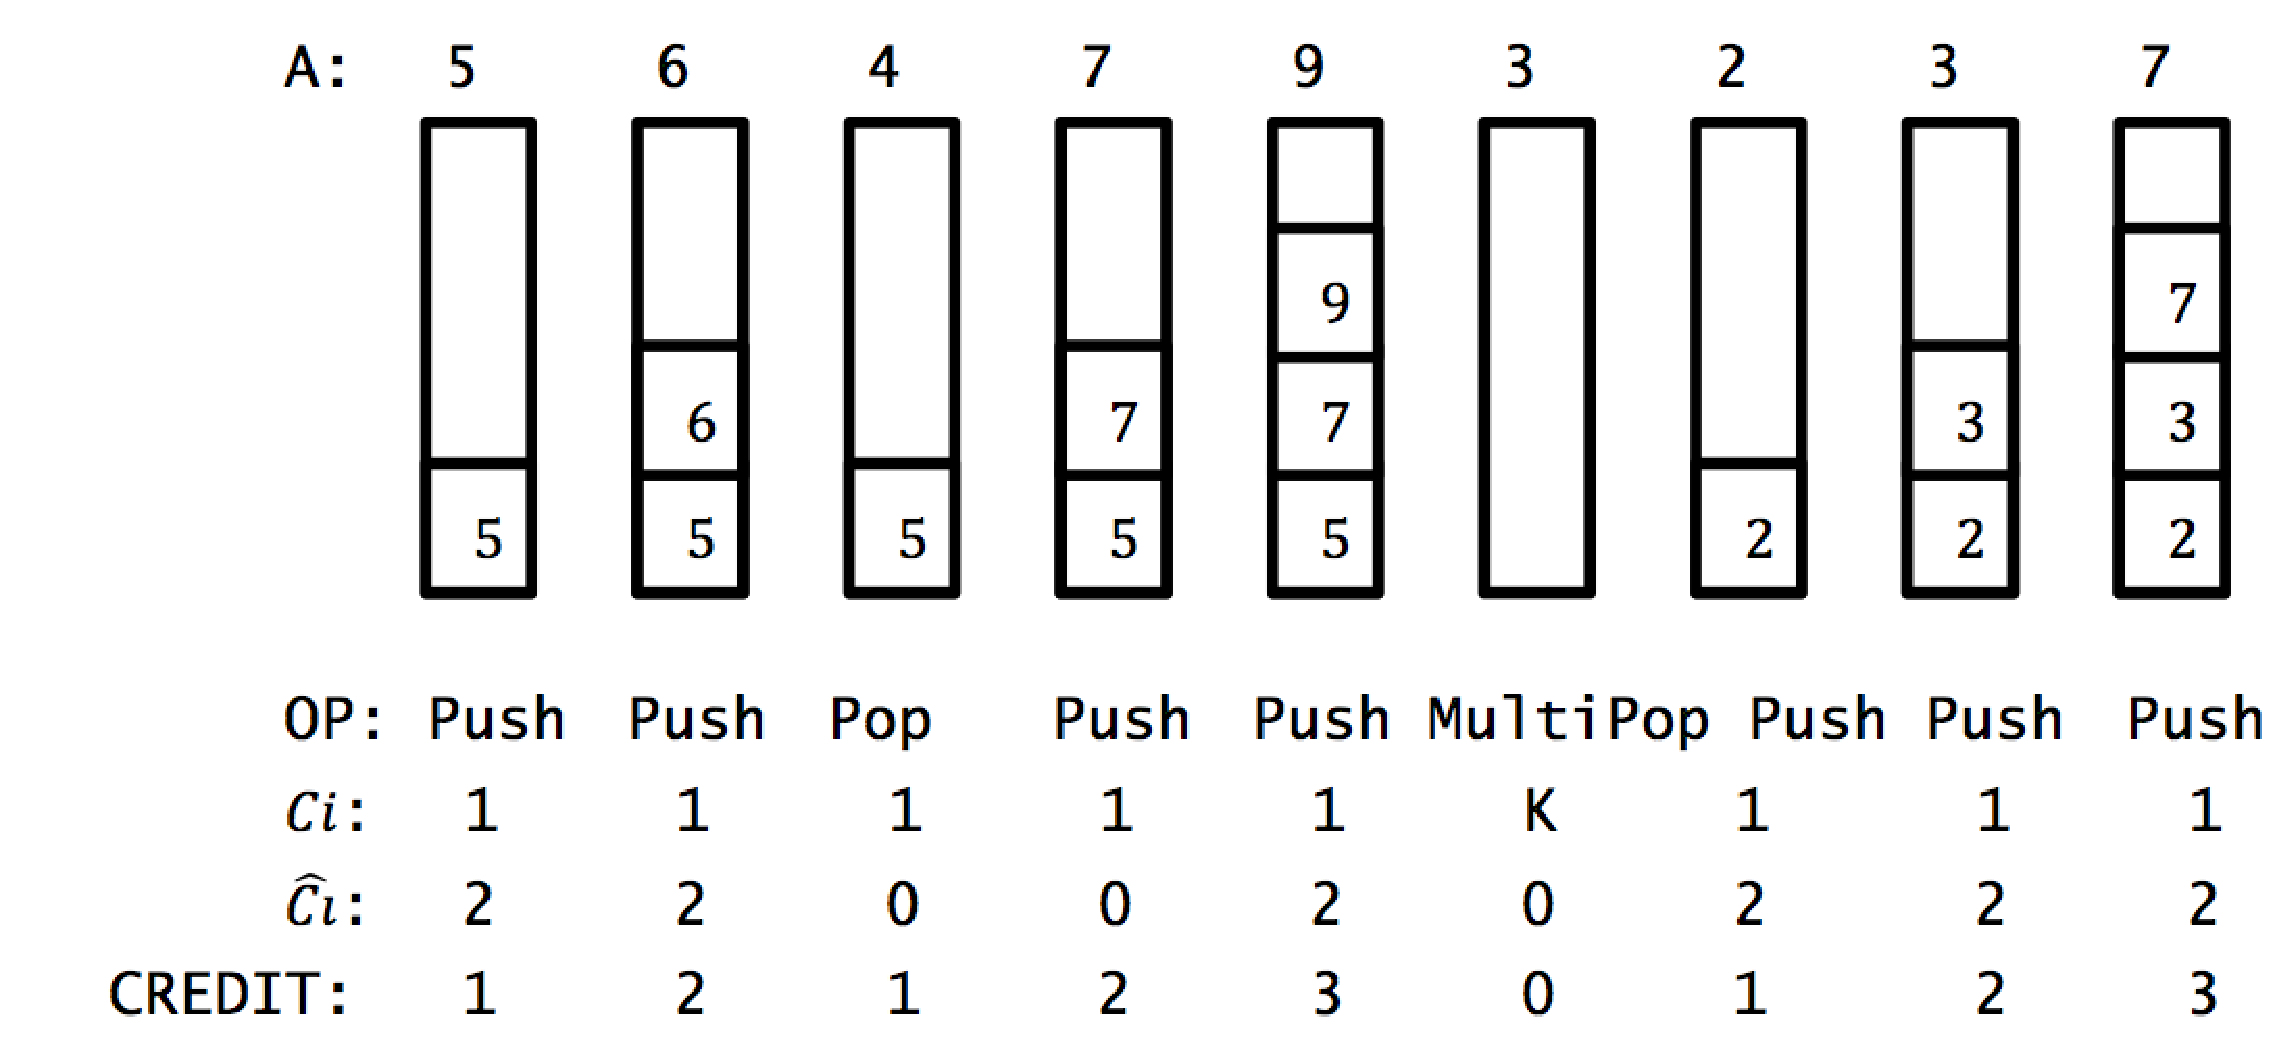
\includegraphics[width=3.5in]{L2-stackexampleaccounting.eps}
\end{figure}
\begin{itemize}
\item Credit: the number of items in the stack. 
\item Constraint: $\sum_{i=1}^n C_i \le  \sum_{i=1}^n \widehat{C_i}$ for arbitrary $n$ operations, i.e. you have enough \textcolor{red}{ {\bf credit}} in your account.\\
\end{itemize}
}


\frame{
	\begin{block}{}
	Tighter analysis 3: potential function technique 
	 \end{block}
}

\frame{
\frametitle{ Tighter analysis 3: Potential technique---``physicisit's view" }
\begin{itemize}
 \item 
Basic idea: sometimes it is not easy to set $\widehat{C_{op}}$ for each operation $OP$ directly. 
\item 
\textcolor{red}{Using potential function as a bridge}, i.e. we assign a value to \textcolor{red}{state} rather than \textcolor{red}{operation}, and  amortized costs are then calculated based on potential function. 
\item 
Potential function: $\Phi(S): S \rightarrow {R}$. Here state $S_i$ refers to the {\sc state} of the stack after the $i$-th operation. 
\item Amortized cost setting:  $ \widehat{C_i} = {C_i} + \Phi(S_i) - \Phi(S_{i-1})$,  \\
\item 
Thus, 
\begin{eqnarray}
 \sum\nolimits_{i=1}^n \widehat{C_i} &=& \sum\nolimits_{i=1}^n ( C_i + \Phi(S_i) - \Phi(S_{i-1}) ) \\
&=& \sum\nolimits_{i=1}^n  C_i + \Phi( S_n) - \Phi( S_0 )
\end{eqnarray}
\item Requirement: To guarantee $\sum_{i=1}^n C_i \le \sum_{i=1}^n \widehat{C_i}$, it suffices to assure  $\Phi( S_n) \ge \Phi( S_0 )$. 
\end{itemize}

}

\frame{
\frametitle{Stack example: Potential changes}
\begin{itemize}
\item 
{\bf Definition:} $\Phi(S)$ denotes the number of items in stack. In fact, we simply \textcolor{red}{\bf use  ``credit'' as potential.} \\
\item 
Correctness: $\Phi(S_{i}) \ge 0 = \Phi(S_0)$ for any $i$; 
\end{itemize} 
 \begin{figure}%
   \begin{center}%
       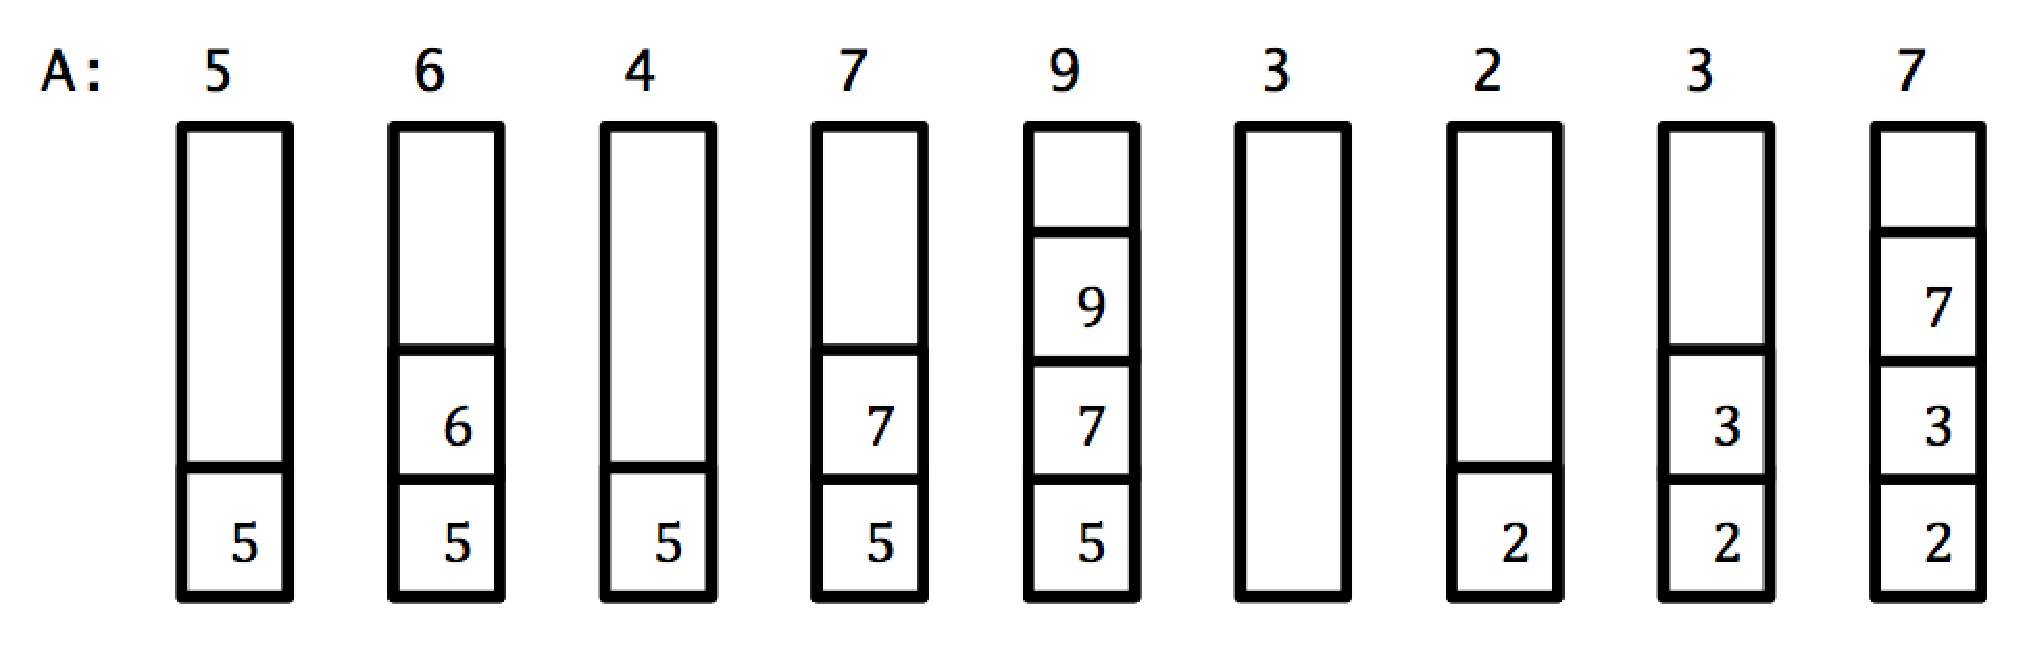
\includegraphics[width=3.in]{L2-stackexamplepotential.eps}%
   \end{center}
 \end{figure}
 \begin{figure}%
   \begin{center}%
      \includegraphics[width=4.0in]{L2-stackexamplepotentialmap.eps}%
   \end{center}
 \end{figure}
}

\frame{
\frametitle{Potential function technique: amortized cost setting }
{\bf Definition:} $\Phi(S)$ denotes the number of items in stack; \\
\begin{itemize}
 \item {\sc Push}: 
 $\Phi(S_i) - \Phi(S_{i-1}) = 1$
\begin{eqnarray}{}
&\widehat{C_i} &=C_i+\Phi(S_i) - \Phi(S_{i-1})\\
	 & &=2
\end{eqnarray}
\item {\sc Pop}: 
$\Phi(S_i) - \Phi(S_{i-1}) = -1$
\begin{eqnarray}
&\widehat{C_i}&=C_i+\Phi(S_i) - \Phi(S_{i-1})\\
	 & &=0
\end{eqnarray}
\item {\sc MultiPop}: 
$\Phi(S_i) - \Phi(S_{i-1}) = -\#Pop $
\begin{eqnarray}
&\widehat{C_i}&=C_i+\Phi(S_i) - \Phi(S_{i-1})\\
	 & &=0
\end{eqnarray}
\item Thus, starting from an empty stack,  \textcolor{red}{ {\bf any sequence}} of $n_{1}$ {\sc Push}, $n_{2}$ {\sc Pop}, and $n_{3}$ {\sc MultiPop}  operations takes at most $T(n) = \sum_{i=1}^n C_i \le   \sum_{i=1}^n \widehat{ C_i} = 2n_{1}$. Here $n=n_{1} + n_{2}  + n_{3}$. 
\end{itemize} 
}

\frame{
	\begin{block}{}
	 {\sc BinaryCounter} problem 
	\end{block}
}

\frame{
\frametitle{{\sc BinaryCounter} problem: incrementing a binary counter}
A sequence of $n$ operations: 
\begin{algorithmic}[1]
\FOR{$i=1$ to $n$} 
\STATE {\sc Increment}(A);
\ENDFOR
\end{algorithmic}

{\sc Increment(A)} \\
\begin{algorithmic}[1]
\STATE $i=0$;
\WHILE{ $i \le A.size() $ AND $ A[i] == 1 $ }
\STATE $A[i] = 0;$
\STATE $i++;$
\ENDWHILE
\IF{$ i \le A.size()$}
\STATE $A[i]=1;$
\ENDIF
\end{algorithmic}

Question: $T(n) \le ?$
}

\frame{
\frametitle{{\sc BinaryCounter} operations: cursory analysis }
\begin{figure}
        \centering
        \includegraphics[width=4in]{L2-binary-counter.eps}
\end{figure}

\begin{itemize}
\item 
Cursory analysis: $T(n) \le kn$ since an increment step might change all $k$ bits. 
\end{itemize}
}


\frame{
	\begin{block}{}
	Tighter analysis 1: aggregate technique 
	 \end{block}
}

\frame{
\frametitle{Tighter analysis 1: Aggregate technique}
\begin{itemize}
 \item Basic operations:  \texttt{flip(1$\rightarrow$0)}, \texttt{flip(0$\rightarrow$1)}
 \begin{eqnarray}
T(n) & = & \sum_{i=1}^n C_i \nonumber \\
     & = & 1 + 2 + 1 + 3 + 1 + 2 + 1 + 4 + ... \nonumber\\
     & = & \#flip\_at\_A0 + \#flip\_at\_A1 + .... + \#flip\_at\_Ak  \nonumber \\ 
     & = & n + \frac{n}{2} + \frac{n}{4} + ...  \nonumber\\
     & \le & 2n \nonumber
\end{eqnarray}
\item Amortized cost of each operation: $O(n)/n=O(1)$.
\end{itemize}
}



\frame{
	\begin{block}{}
	Tighter analysis 2: accounting technique 
	 \end{block}
}

\frame{
\frametitle{Tighter analysis 2: Accounting technique}

Set amortized cost as follows: 
\begin{table}
	\begin{tabular}{c|cc} 
	$OP$ & Real Cost $C_{OP}$ & Amortized Cost $\widehat{C_{OP}}$ \\ \hline
	\texttt{flip(0$\rightarrow$1)} & 1 & 2 \\
	\texttt{flip(1$\rightarrow$0)} & 1 & 0 
	\end{tabular} 
\end{table} 

%\begin{figure}
%        \centering
%        \includegraphics[width=2in]{L2-incrementaccounting.eps}
%\end{figure}
Key observation: $ \#flip(0\rightarrow1) \ge \#flip(1\rightarrow0)$
 \begin{eqnarray}
T(n) & = & \sum_{i=1}^n C_i \\
     & = & \#flip(0\rightarrow1) + \#flip(1\rightarrow0) \\ 
     & \le & 2 \#flip(0\rightarrow1) \\
     & \le & 2n
\end{eqnarray}
}


\frame{
	\begin{block}{}
	Tighter analysis 3: potential function technique 
	 \end{block}
}

\frame{
\frametitle{Tighter analysis 3: Potential function technique}
 
{\bf Definition:} Set potential function as $\Phi(S)$ = \#1 in counter\\
 \begin{figure}%
   \begin{center}%
      \includegraphics[width=3.0in]{L2-binary-counter.eps}%
   \end{center}
 \end{figure}
 \begin{figure}%
   \begin{center}%
      \includegraphics[width=4.2in]{L2-incrementpotentialmap.eps}%
   \end{center}
 \end{figure}
}

\frame{
\frametitle{Tighter analysis: Potential technique   cont'd}
\begin{itemize}
 \item {\bf Definition:}  Set potential function as $\Phi(S)$ = \#1 in counter; \\
 \item At step $i$, the number of flips $C_i$ is: 
 \begin{eqnarray}
 C_i  &=& \#flip^{(i)}_{0\rightarrow 1} + \#flip^{(i)}_{1\rightarrow 0} = 1 + \#flip^{(i)}_{1\rightarrow 0}  \quad (why?)  \nonumber \\
\Phi(S_i) &=& \Phi(S_{i-1}) + 1 - \#flip^{(i)}_{1\rightarrow 0} \nonumber \\
 \widehat{C_i} &=& C_i + \Phi(S_i) - \Phi(S_{i-1})     \nonumber  \\ 
      & \le & 2 \nonumber 
\end{eqnarray}
\item 
Thus we have
\begin{eqnarray}
T(n) &=& \sum\nolimits_{i=1}^n C_i \nonumber \\ 
     &\le& \sum\nolimits_{i=1}^n \widehat{C_i} \nonumber \\
     &\le& 2n \nonumber
\end{eqnarray}
\item In other words, starting from $00....0$, a sequence of $n$ {\sc Increment} operations takes at most $2n$ time. 
\end{itemize}

}

% \begin{figure}
%         \centering
%         \includegraphics[width=2in]{L2-incrementaccounting.eps}
% \end{figure}
% Key observation: $ \#flip(0\rightarrow1) >= \#flip(1\rightarrow0)$
%   \begin{eqnarray}
% T(n) & = & \sum_{i=1}^n C_i \\
%      & = & \#flip(0\rightarrow1) + \#flip(1\rightarrow0) \\ 
%      & <= & 2 \#flip(0\rightarrow1) \\
%      & <= & 2n
% \end{eqnarray}
% }
\frame{
	\begin{block}{}
	{\sc DynamicTable} problem
	\end{block}
}

\frame{
\frametitle{ A practical problem  }
Practical problem: 
\begin{itemize}
\item Suppose you are asked to develop a  {\tt C++} compiler.
\item {\tt vector} is one of a {\tt C++}  class templates to hold a set of objects. It supports the following operations: 
\begin{itemize}
	\item {\tt push\_back}: to add a new object onto the tail; 
	\item {\tt pop\_back}: to pop out the last object; 
\end{itemize}
\item Recall that {\tt vector} uses a \textcolor{blue}{\bf contiguous memory area} to store objects. 
\item Question: How to design an efficient \textcolor{blue}{\bf memory-allocation strategy} for {\tt vector}? 
\end{itemize} 
}

\frame{
\frametitle{ {\sc DynamicTable} problem  }

\begin{itemize}
	\item In many applications, we do not know in advance how many objects will be stored in a table. 
	\item  Thus we have to allocate space for a table, only to find out later that it is not enough. 
	\item \textcolor{blue}{\sc Dynamic Expansion:} When inserting a new item into a full table, the table must be reallocated with a larger size, and the objects in the original table must be copied into the new table. 
	\item \textcolor{blue}{\sc Dynamic Contraction:} Similarly, if many objects have been removed from a table, it is worthwhile to reallocate the table with a smaller size. 
	\item We will show a \textcolor{blue}{\bf memory allocation strategy} such that the amortized cost of insertion and deletion is $O(1)$, even if the actual cost of an operation is large when it triggers an expansion or contraction.  
\end{itemize} 
} 


\frame{
	\begin{block}{}
	{\sc DynamicTable} supporting {\sc TableInsertion} operation only
	\end{block}	
}


\frame{
	\frametitle{Double-size strategy} 

{\sc Table\_Insert}$(T, i)$
	\begin{algorithmic}[1]
	\IF{$size[T]==0$} 
	\STATE{ allocate a table with $1$ slot; } 
	\STATE{ $size[T]=1;$ }
	\ENDIF
	\IF{$num[T]==size[T]$  }  
	\STATE{ allocate a new table with $2\times size[T]$ slots; //\textcolor{red}{\bf double size} }
	\STATE{ $size[T]=2\times size[T]$; }
	\STATE{ copy all items into the new table; }
	\STATE{ free the original table; }
	\ENDIF
	\STATE{ insert the new item $i$ into $T$; } 
	\STATE{  $num[T]++$; }
	\end{algorithmic}
 \begin{figure}%
   \begin{center}%
         \includegraphics[width=2.2in]{L2-vector.eps}%
     \end{center}
 \end{figure}
	
}


\frame{
	\frametitle{Example: {\sc TableInsert(1)}  }
	Consider a sequence of operations starting with an empty table: 
	\begin{algorithmic}[1]
	\STATE{ Table $T$;}
	\FOR{$i = 1$ to $n$ }
	\STATE{  {\sc Table\_Insert}$(T, i);$ }
	\ENDFOR
	\end{algorithmic}
	
 \begin{figure}%
   \begin{center}%
         \includegraphics[width=3in]{L2-tableinsertstep1.eps}%
     \end{center}
 \end{figure}
	
}

\frame{
	\frametitle{ {\sc TableInsert(2)} }
 \begin{figure}%
   \begin{center}%
         \includegraphics[width=3in]{L2-tableinsertstep2.eps}%
     \end{center}
 \end{figure}
}

\frame{
	\frametitle{ {\sc TableInsert(2)} }
 \begin{figure}%
   \begin{center}%
         \includegraphics[width=3in]{L2-tableinsertstep21.eps}%
     \end{center}
 \end{figure}
}

\frame{
	\frametitle{ {\sc TableInsert(2)} }
 \begin{figure}%
   \begin{center}%
         \includegraphics[width=3in]{L2-tableinsertstep22.eps}%
     \end{center}
 \end{figure}
}

\frame{
	\frametitle{ {\sc TableInsert(2)} }
 \begin{figure}%
   \begin{center}%
         \includegraphics[width=3in]{L2-tableinsertstep23.eps}%
     \end{center}
 \end{figure}
}


\frame{
	\frametitle{ {\sc TableInsert(3)} }
 \begin{figure}%
   \begin{center}%
         \includegraphics[width=3in]{L2-tableinsertstep3.eps}%
     \end{center}
 \end{figure}
}

\frame{
	\frametitle{ {\sc TableInsert(3)} }
 \begin{figure}%
   \begin{center}%
         \includegraphics[width=3in]{L2-tableinsertstep31.eps}%
     \end{center}
 \end{figure}
}

\frame{
	\frametitle{ {\sc TableInsert(3)} }
 \begin{figure}%
   \begin{center}%
         \includegraphics[width=3in]{L2-tableinsertstep32.eps}%
     \end{center}
 \end{figure}
}

\frame{
	\frametitle{ {\sc TableInsert(3)} }
 \begin{figure}%
   \begin{center}%
         \includegraphics[width=3in]{L2-tableinsertstep33.eps}%
     \end{center}
 \end{figure}
}

\frame{
	\frametitle{ {\sc TableInsert(4)} }
 \begin{figure}%
   \begin{center}%
         \includegraphics[width=3in]{L2-tableinsertstep4.eps}%
     \end{center}
 \end{figure}
}


\frame{
	\frametitle{ {\sc TableInsert(5)} }
 \begin{figure}%
   \begin{center}%
         \includegraphics[width=3in]{L2-tableinsertstep5.eps}%
     \end{center}
 \end{figure}
}

\frame{
	\frametitle{ {\sc TableInsert(5)} }
 \begin{figure}%
   \begin{center}%
         \includegraphics[width=3in]{L2-tableinsertstep51.eps}%
     \end{center}
 \end{figure}
}

\frame{
	\frametitle{ {\sc TableInsert(5)} }
 \begin{figure}%
   \begin{center}%
         \includegraphics[width=3in]{L2-tableinsertstep52.eps}%
     \end{center}
 \end{figure}
}

\frame{
	\frametitle{ {\sc TableInsert(5)} }
 \begin{figure}%
   \begin{center}%
         \includegraphics[width=3in]{L2-tableinsertstep53.eps}%
     \end{center}
 \end{figure}
}


\frame{
	\frametitle{Cursory analysis: $O(n^2)$ }
		\begin{itemize}
		\item 
	Consider a sequence of operations starting with an empty table: 
	\begin{algorithmic}[1]
	\STATE{ Table $T$;}
	\FOR{$i = 1$ to $n$ }
	\STATE{  {\sc Table\_Insert}$(T, i);$ }
	\ENDFOR
	\end{algorithmic}

	\item What is the actual cost $C_i$ of the $i$th operation? \footnote{Here the cost is measured in terms of elementary insertions or deletions. }
	 $C_i = \begin{cases} 
	                 i &  \text{if } i-1 \text{ is an exact power of 2} \\ 
	                 1 & \text{otherwise}\\
	                  \end{cases} $
	\item Here $C_i=i$ when the table is full, since we need to perform 1 insertion, and copy $i-1$ items into the new table.
	\item If $n$ operations are performed, the worst-case cost of an operation will be  $O(n)$. 
	\item Thus, the total running time for a total of $n$ operations is $O(n^2)$.  \textcolor{red}{\bf Not tight!}
	\end{itemize}
	
} 


\frame{
	\begin{block}{}
		Tighter analysis 1: Aggregate technique 
	\end{block}
}

\frame{
	\frametitle{Aggregate method: {\bf table expansions} are rare } 
	\begin{itemize}
	\item The $O(n^2)$ bound is not tight since \textcolor{blue}{\bf table expansion}  doesn't occur often in the course of $n$ operations. 
	\item Specifically, \textcolor{blue}{\bf table expansion} occurs at the $i$th operation, where $i-1$ is an exact power of $2$.
	 $C_i = \begin{cases} 
	                 i &  \text{if } i-1 \text{ is an exact power of 2} \\ 
	                 1 & \text{otherwise}\\
	                  \end{cases} $
	\end{itemize}
	
	   \begin{figure}%
   \begin{center}%
         \includegraphics[width=4in]{L2-table-insert-ci2.eps}%
     \end{center}
 \end{figure}
}


\frame{
	\frametitle{ Aggregate method: rewriting $C_i$} 
	\begin{itemize}
	\item The $O(n^2)$ bound is not tight since  {\bf table expansion}  doesn't occur often in the course of $n$ operations. 
	\item Specifically, {\bf table expansion} occurs at the $i$th operation, where $i-1$ is an exact power of $2$.
	 $C_i = \begin{cases} 
	                 i &  \text{if } i-1 \text{ is an exact power of 2} \\ 
	                 1 & \text{otherwise}\\
	                  \end{cases} $

	\item We decompose $C_i$ as follows: 
	\begin{figure}%
   \begin{center}%
         \includegraphics[width=4in]{L2-table-insert-ci1.eps}%
     \end{center}
 \end{figure}
      	\end{itemize}
}

\frame{
	\frametitle{Total cost of $n$ operations}
	 \begin{itemize}
	 	\item The total cost of $n$ operations is: 
		\begin{eqnarray}
			\sum_{i=1}^n C_i & = &  1 + 2 + 3 + 1 + 5 + 1 + 1 + 1 + 9 + 1+ ... \nonumber \\
			                            & = &  n + \sum_{j=0}^{ \lfloor \lg n \rfloor }  2^j  \nonumber \\ 
			                            & < &  n  + 2n \nonumber \\ 
			                            & = & 3n \nonumber             
		\end{eqnarray}
		\item Thus the amortized cost of an operation is 3. 
		\item In other words, the average cost of each {\sc TableInsert} operation is $O(n)/n=O(1)$. 
	 \end{itemize}
}



\frame{
	\begin{block}{}
		Tighter analysis 2: Accounting technique 
	\end{block}
}


\frame{
	\frametitle{ Tighter analysis 2: accounting technique } 
	\begin{itemize}
	\item  For the $i$-th operation, an \textcolor{blue}{\bf amortized cost} $\widehat{C_{i}}=\$3$ is charged. 	
	\item This fee is consumed to perform subsequent operations. 
	\item Any amount not immediately consumed is stored in a "bank" for use for subsequent operations. 
	\item Thus for the $i$-th insertion, the $\$3$ is used as follows: 
		\begin{itemize}
			\item $\$ 1$ pays for the insertion \textcolor{blue}{\bf itself}; 
			\item $\$ 2$ is stored for \textcolor{blue}{\bf later table doubling}, including $\$ 1$ for copying one of the recent $\frac{i}{2}$ items, and $\$ 1$ for copying one of the old $\frac{i}{2}$ items. 
		\end{itemize}
	\end{itemize}
	
 \begin{figure}%
   \begin{center}%
         \includegraphics[width=2in]{L2-tableinsert-accounting1.eps}%
     \end{center}
 \end{figure}
	
	
} 


\frame{
	\frametitle{ Tighter analysis 2: accounting technique } 
	\begin{itemize}
	\item  For the $i$-th operation, an \textcolor{blue}{\bf amortized cost} $\widehat{C_{i}}=\$3$ is charged. 	
	\item This fee is consumed to perform the operation. 
	\item Any amount not immediately consumed is stored in a "bank" for use for subsequent operations. 
	\item Thus for the $i$-th insertion, the $\$3$ is used as follows: 
		\begin{itemize}
			\item $\$ 1$ pays for the insertion \textcolor{blue}{\bf itself}; 
			\item $\$ 2$ is stored for \textcolor{blue}{\bf later table doubling}, including $\$ 1$ for copying one of the recent $\frac{i}{2}$ items, and $\$ 1$ for copying one of the old $\frac{i}{2}$ items. 
		\end{itemize}
	\end{itemize}
	
 \begin{figure}%
   \begin{center}%
         \includegraphics[width=4in]{L2-tableinsert-accounting2.eps}%
     \end{center}
 \end{figure}
	
	
} 



\frame{
	\frametitle{ Tighter analysis 2: accounting technique } 
	\begin{itemize}
	\item  Key observation: the credit never goes negative. In other words, the sum of amortized cost provides an upper bound of the sum of actual costs. 
	\begin{eqnarray} 
		T(n) & = & \sum_{i=1}^n C_i \nonumber \\ 
		        & \leq & \sum_{i=1}^n \widehat{ C_i } \nonumber \\ 
		        & = & 3n \nonumber  
	\end{eqnarray}	        
	\end{itemize}
	
 \begin{figure}%
   \begin{center}%
         \includegraphics[width=4in]{L2-tableinsert-accounting3.eps}%
     \end{center}
 \end{figure}
	
	
} 



\frame{
	\begin{block}{}
		Tighter analysis 3: Potential function technique 
	\end{block}
}


\frame{
	\frametitle{ Tighter analysis 3: potential function technique  } 
	\begin{itemize}
	\item Motivation: sometimes it is not easy to find an appropriate amortized cost \textcolor{blue}{\bf directly}. An alternative way is to use a \textcolor{blue}{\bf potential function} as a bridge.
	\item Basic idea: the  \textcolor{blue}{\bf bank account} can be viewed as  potential function of the dynamic set.  More specifically, we prefer a potential function $\Phi: \{ T \} \rightarrow  R $ with  the following properties: 
		\begin{itemize}
			\item $\Phi(T) = 0$ immediately \textcolor{blue}{\bf after} an expansion; 
			\item $\Phi(T) = size[T]$ immediately \textcolor{blue}{\bf before} an expansion; thus, the next expansion can be paid for by the potential. 
		\end{itemize}
	\item A possibility:  $\Phi(T) = 2 \times num[T] - size[T]$
	\end{itemize}
 \begin{figure}%
   \begin{center}%
         \includegraphics[width=2.4in]{L2-tableinsert-potential-accounting.eps}%
     \end{center}
 \end{figure}
} 

\frame{
	\frametitle{ $\Phi(T) = 2 \times num[T] - size[T]$: an example}
 \begin{figure}%
   \begin{center}%
         \includegraphics[width=4.in]{L2-tablephi1.eps}%
     \end{center}
     \caption{ The effect of a sequence of $n$ {\sc TableInsert} on $size_{i}$ (red), $num_{i}$ (green), and $\Phi_{i}$ (blue). }
 \end{figure}
}

\frame{
	\frametitle{ Correctness of  $\Phi(T) = 2 \times num[T] - size[T]$}
	\begin{itemize}
		 
	\item Correctness: Initially $\Phi_0=0$, and it is easy to verify that $\Phi_i \geq \Phi_0$ since the table is always at least half full. 
		\item The \textcolor{blue}{\bf amortized cost} $\widehat{ C_i}$ with respect to $\Phi$ is defined as: 
			$\widehat{ C_i } = C_i + \Phi(T_i) - \Phi(T_{i-1})$. 
		\item Thus $\sum_{i=1}^n \widehat{C_i} =  \sum_{i=1}^n {C_i} + \Phi_n - \Phi_0$  is really an upper bound of the actual cost $ \sum_{i=1}^n {C_i}$.
	\end{itemize}

 } 



\frame{
	\frametitle{ Calculate $\widehat{C_i}$ with respect to $\Phi$ }
	
	\begin{itemize}
		\item Case 1: the $i$-th insertion does not trigger an expansion
		\item Then $size_{i} = size_{i-1}$.  Here,  $num_i$ denotes the number of items after the $i$-th operations, $size_i$ denotes the table size, and $T_i$ denotes the potential.
		\begin{eqnarray}
			\widehat{C_i} & = & C_i + \Phi_i - \Phi_{i-1} \nonumber \\ 
					& = & 1 + (2 num_i - size_i) - (2 num_{i-1} - size_{i-1}) \nonumber \\ 
					& = & 1 + 2 \nonumber \\ 
					& = & 3 \nonumber
		\end{eqnarray}
	\end{itemize}
  \begin{figure}%
   \begin{center}%
         \includegraphics[width=3in]{L2-tableinsertstep4.eps}%
     \end{center}
 \end{figure}
}


\frame{
	\frametitle{ Calculate $\widehat{C_i}$ with respect to $\Phi$ }
		\begin{itemize}
		\item Case 2: the $i$-th insertion triggers an expansion
		\item Then $size_{i} = 2 \times size_{i-1} $. 
		\begin{eqnarray}
			\widehat{C_i} & = & C_i + \Phi_i - \Phi_{i-1} \nonumber \\ 
					& = & num_i + (2 num_i - size_i) - (2 num_{i-1} - size_{i-1}) \nonumber \\ 
					& = & num_i + 2 - (num_i - 1)   \nonumber \\ 
					& = & 3 \nonumber
		\end{eqnarray}
	\end{itemize}
	  \begin{figure}%
   \begin{center}%
         \includegraphics[width=3in]{L2-tableinsertstep53.eps}%
     \end{center}
 \end{figure}
} 
\frame{
	\frametitle{Conclusion}
	\begin{block}{}
	 Starting with an empty table, a sequence of $n$ {\sc TableInsert} operations cost $O(n)$ time in the worst case. 
\end{block}{}
}


\frame{
	\begin{block}{}
	{\sc DynamicTable} supporting {\sc TableInsert} and {\sc TableDelete}
	\end{block}	
}

\frame{
	\frametitle{ {\sc TableDelete} operation } 
	\begin{itemize}
		\item To implement {\sc TableDelete} operation, it is simple to remove the specified item from the table, followed by a {\sc Contraction} operation when the \textcolor{blue}{\bf load factor} (denoted as $\alpha(T)=\frac{num[T]}{size[T]}$) is small, so that the wasted space is not exorbitant. 
		\item Specifically, when the number of the items in the table drops too low, we allocate a new, smaller space,  copy the items from the old table to the new one, and finally free the original table. 
		\item We would like the following two properties: 
			\begin{enumerate}
				\item The load factor is bounded below  by a constant; 
				\item The amortized cost of a table  operation is bounded above by a constant. 
			\end{enumerate}
	\end{itemize}
}

\frame{
	\begin{block}{}
	Trial 1:  load factor $\alpha(T)$ never drops below 1/2
	\end{block}
}

\frame{
	\frametitle{Trial 1: load factor $\alpha(T)$ never drops below 1/2}
	\begin{itemize}
	\item A natural strategy is:
		\begin{itemize}
			\item To double the table size when inserting an item into a full table; 
			\item To halve the table size when deletion causes $\alpha(T)<\frac{1}{2}$. 
		\end{itemize}
	\item The strategy guarantees that  load factor $\alpha(T)$ never drops below 1/2. 
	\item However, the amortized cost of an operation might be quite large. 
	\end{itemize}
}


\frame{
	\frametitle{An example of large amortized cost}
	\begin{itemize}
		\item Consider a sequence of $n=16$ operations: 
		\begin{itemize}
			\item The first $8$ operations: {\tt I, I, I,....}
			\item The second  $8$ operations: {\tt I, D, D, I, I, D, D, I, I,...}
		\end{itemize}
		\item Note: 
			\begin{itemize}
			\item After the $8$-th {\tt I}, we have $num_{16} = size_{16} = 16$.
			\item The $9$-th {\tt I} leads to a table expansion; 
			\item The following two {\tt D} lead to a table contraction; 
			\item The following two {\tt I} lead to a table expansion, and so on. 
			\end{itemize}
		\end{itemize}
		\begin{figure}
			\includegraphics[width=2.5in]{L2-tableinsertdelete.eps}
		\end{figure} 
} 

\frame{
	\frametitle{An example of large amortized cost}
		\begin{figure}
			\includegraphics[width=2.5in]{L2-tableinsertdelete.eps}
		\end{figure} 
	\begin{itemize}
			\item The expansion/contraction takes $O(n)$ time, and there are $n$ of them. 
		\item Thus the total cost of $n$ operations are $O(n^{2})$, and the amortized cost of an operation is $O(n)$. 
	\end{itemize}
}


\frame{
	\begin{block}{}
	Trial 2:  load factor $\alpha(T)$ never drops below 1/4
	\end{block}
}

\frame{
	\frametitle{Trial 1: load factor $\alpha(T)$ never drops below 1/2}
	\begin{itemize}
	\item Another strategy is:
		\begin{itemize}
			\item To double the table size when inserting an item into a full table; 
			\item To halve the table size when deletion causes $\alpha(T)<\frac{1}{4}$. 
		\end{itemize}
	\item The strategy guarantees that  load factor $\alpha(T)$ never drops below 1/4. 
	\end{itemize}
}

\frame{
	\frametitle{Amortized analysis}
	\begin{itemize}
		\item We start by defining a potential function $\Phi(T)$ that is $0$ immediately after an expansion or contraction, and builds as $\alpha(T)$ increases to $1$ or decreases to $\frac{1}{4}$. 
		$\Phi(T)=\begin{cases} 
				2\times num[T] - size[T] & \texttt{if } \alpha(T)\geq \frac{1}{2}\\
				\frac{1}{2}size[T] - num[T] &  \texttt{if } \alpha(T)\leq \frac{1}{2} 
				\end{cases}$
		\item Correctness: the potential is $0$ for an empty table, and $\Phi(T)$ never goes negative. Thus, the total amortized cost of a sequence of $n$ operations with respect to $\Phi$ is an upper bound of the actual cost. 
	\end{itemize}
}

\frame{
	\begin{block}{}
	Amortized cost of {\sc TableInsert} operation
	\end{block}
}

\frame{
	\frametitle{Amortized cost of {\sc TableInsert} }
	\begin{itemize}
	\item 	Case 1: $\alpha_{i-1} \geq \frac{1}{2}$ and no expansion
		\item The amortized cost is: 
		\begin{eqnarray}
			\widehat{C_{i}} &=& C_{i} + \Phi_{i} - \Phi_{i-1} \nonumber \\ 
						&=& 1 + ( 2num_{i} - size_{i}) - ( 2num_{i-1}  - size_{i-1}) \nonumber \\
						&=& 1 + ( 2(num_{i-1}+1) - size_{i}) - ( 2num_{i-1}  - size_{i}) \nonumber \\
						&=& 3 \nonumber 
		\end{eqnarray}
	\end{itemize}
		  \begin{figure}%
   \begin{center}%
         \includegraphics[width=3in]{L2-tableinsertstep4.eps}%
     \end{center}
 \end{figure}
}


\frame{
	\frametitle{Amortized cost of {\sc TableInsert} }
	\begin{itemize}
	\item Case 2: $\alpha_{i-1} \geq \frac{1}{2}$ and an expansion was triggered
	\item The amortized cost is: 
		\begin{eqnarray}
			\widehat{C_{i}} &=& C_{i} + \Phi_{i} - \Phi_{i-1} \nonumber \\ 
						&=& num_{i} + ( 2num_{i} - size_{i}) - ( 2num_{i-1}  - size_{i-1}) \nonumber \\
						&=& num_{i-1} + 1 + ( 2(num_{i-1}+1) - 2 size_{i-1}) - (2num_{i-1}  - size_{i-1}) \nonumber \\
						&=& 3 + num_{i-1} - size_{i-1} \nonumber  \\
						&=& 3 \nonumber 
		\end{eqnarray}
	\end{itemize}
		  \begin{figure}%
   \begin{center}%
         \includegraphics[width=3in]{L2-tableinsertstep53.eps}%
     \end{center}
 \end{figure}
}


\frame{
	\frametitle{Amortized cost of {\sc TableInsert} }
		\begin{itemize}
\item 	Case 3: $\alpha_{i-1} < \frac{1}{2}$  and $\alpha_{i} < \frac{1}{2}$
		\item The amortized cost is: 
		\begin{eqnarray}
			\widehat{C_{i}} &=& C_{i} + \Phi_{i} - \Phi_{i-1} \nonumber \\ 
						&=& 1 + ( \frac{1}{2} size_{i} - num_{i} ) - (\frac{1}{2} size_{i-1} - num_{i-1}) \nonumber \\
						&=& 1 + ( \frac{1}{2} size_{i} - num_{i} ) - (\frac{1}{2} size_{i} - (num_{i} -1)) \nonumber \\
						&=& 0 \nonumber 
		\end{eqnarray}
	\end{itemize}
			  \begin{figure}%
   \begin{center}%
         \includegraphics[width=3in]{L2-tableinsert-case3.eps}%
     \end{center}
 \end{figure}
}

\frame[allowframebreaks]{
	\frametitle{Amortized cost of {\sc TableInsert} }
	
	\begin{itemize}
		\item Case 4: $\alpha_{i-1} < \frac{1}{2}$  but $\alpha_{i} \geq \frac{1}{2}$
		\item The amortized cost is: 
		\begin{eqnarray}
			\widehat{C_{i}} &=& C_{i} + \Phi_{i} - \Phi_{i-1} \nonumber \\ 
						&=& 1 + ( 2 num_{i} - size_{i}  ) - (\frac{1}{2} size_{i-1} - num_{i-1}) \nonumber \\
						&=& 1 + ( 2  (num_{i-1}+1) - size_{i-1} ) - (\frac{1}{2} size_{i-1} - num_{i-1}) \nonumber \\
						&=& 3  num_{i-1}  - \frac{3}{2} size_{i-1} +3  \nonumber \\
						&=& 3 \alpha_{i-1}num_{i-1}  - \frac{3}{2} size_{i-1} +3  \nonumber \\
						&<& \frac{3}{2} size_{i-1} - \frac{3}{2} size_{i-1} + 3  \nonumber \\ 
						&=& 3 \nonumber 
		\end{eqnarray}
	\end{itemize}
				  \begin{figure}%
   \begin{center}%
         \includegraphics[width=3in]{L2-tableinsert-case4.eps}%
     \end{center}
 \end{figure}
}



\frame{
	\begin{block}{}
	Amortized cost of {\sc TableDelete} operation
	\end{block}
}

\frame{
	\frametitle{Amortized cost of {\sc TableDelete} }
	\begin{itemize}
	\item 	Case 1: $\alpha_{i-1} < \frac{1}{2}$ and no contraction 
		\item The amortized cost is: 
		\begin{eqnarray}
			\widehat{C_{i}} &=& C_{i} + \Phi_{i} - \Phi_{i-1} \nonumber \\ 
						&=& 1 + ( \frac{1}{2} size_{i} - num_{i} ) - (\frac{1}{2} size_{i-1} - num_{i-1}) \nonumber \\
						&=& 1 + ( \frac{1}{2} size_{i-1} - (num_{i-1}-1) ) - (\frac{1}{2} size_{i-1} - num_{i-1}) \nonumber \\
						&=& 2\nonumber 
		\end{eqnarray}
	\end{itemize}
\begin{figure}%
	   \begin{center}%
         \includegraphics[width=3in]{L2-tabledelete-case1.eps}%
     \end{center}
 \end{figure}
}

\frame{
	\frametitle{Amortized cost of {\sc TableDelete} }
	\begin{itemize}
	\item 	Case 2: $\alpha_{i-1} < \frac{1}{2}$ and a contraction was triggered
	\item The amortized cost is: 
		\begin{eqnarray}
			\widehat{C_{i}} &=& C_{i} + \Phi_{i} - \Phi_{i-1} \nonumber \\ 
						&=& num_{i} + 1 + ( \frac{1}{2} size_{i} - num_{i} ) - (\frac{1}{2} size_{i-1} - num_{i-1}) \nonumber \\
						&=&  num_{i-1}  + ( \frac{1}{4} size_{i-1} - (num_{i-1}-1) ) - (\frac{1}{2} size_{i-1} - num_{i-1}) \nonumber \\
						&=& 1 + num_{i-1} - \frac{1}{4} size_{i-1} \nonumber \\
						&=& 1 \nonumber 
		\end{eqnarray}
	\end{itemize}
	
	\begin{figure}%
	   \begin{center}%
         \includegraphics[width=3in]{L2-tabledelete-case2.eps}%
     \end{center}
 \end{figure}

}

\frame{
	\frametitle{Amortized cost of {\sc TableInsert} }
	\begin{itemize}
	\item Case 3: $\alpha_{i-1} \geq \frac{1}{2}$ and $\alpha_{i} \geq \frac{1}{2}$
	\item The amortized cost is: 
		\begin{eqnarray}
			\widehat{C_{i}} &=& C_{i} + \Phi_{i} - \Phi_{i-1} \nonumber \\ 
						&=& 1 + ( 2num_{i} - size_{i}) - ( 2num_{i-1}  - size_{i-1}) \nonumber \\
						&=& 1 + ( 2(num_{i-1}+1) - size_{i-1}) - (2num_{i-1}  - size_{i-1}) \nonumber \\
						&=& 3 \nonumber 
		\end{eqnarray}
	\end{itemize}
	\begin{figure}%
	   \begin{center}%
         \includegraphics[width=3in]{L2-tabledelete-case3.eps}%
     \end{center}
 \end{figure}

}


\frame{
	\frametitle{Amortized cost of {\sc TableInsert} }
	\begin{itemize}
	\item Case 4: $\alpha_{i-1} \geq \frac{1}{2}$ and $\alpha_{i} < \frac{1}{2}$
	\item The amortized cost is: 
		\begin{eqnarray}
			\widehat{C_{i}} &=& C_{i} + \Phi_{i} - \Phi_{i-1} \nonumber \\ 
						&=& 1 + ( \frac{1}{2} size_{i} - num_{i} ) - ( 2num_{i-1}  - size_{i-1} ) \nonumber \\
						&=& 1 + ( \frac{1}{2} size_{i-1} - (num_{i-1}-1) ) - (2num_{i-1}  - size_{i-1}) \nonumber \\
						&=& 2 + \frac{3}{2} size_{i-1} - 3 num_{i-1} \nonumber \\
						&\leq&  2 \nonumber 
		\end{eqnarray}
	\end{itemize}
	\begin{figure}%
	   \begin{center}%
         \includegraphics[width=3in]{L2-tabledelete-case4.eps}%
     \end{center}
 \end{figure}

}

\frame{
	\frametitle{Conclusion}
	\begin{block}{}
		In summary, since the amortized cost of each operation is bounded above by a constant,  
 the actual cost of \textcolor{red}{any sequence of $n$} {\sc TableInsert} and {\sc TableDelete} operations on a dynamic table is $O(n)$ if starting with an empty table.  
	\end{block}
}

\frame{
\frametitle{More examples}
We will talk about the following examples later: 
\begin{itemize}
	\item Binomial heap and Fibonacci heap
	\item Splay-tree
	\item Union-Find 
\end{itemize}
}
\end{document}
